% UTF-8. Compile twice with XeLaTeX from this directory.
% On systems without Windows fonts, replace fontset=windows by fontset=fandol.
\documentclass[UTF8,a4paper,zihao=-4,fontset=windows]{ctexart}
\usepackage[margin=24mm,headheight=15pt]{geometry}
\usepackage{amsmath,amssymb,amsthm,mathtools,graphicx,booktabs,enumitem,fancyhdr,float,placeins}
\usepackage[unicode,colorlinks=true,linkcolor=black,citecolor=black,urlcolor=blue]{hyperref}
\linespread{1.08}
\setlength{\parskip}{.15em}
\setlength{\emergencystretch}{2em}
\setlist{itemsep=.15em,topsep=.4em}
\ctexset{section={format=\Large\bfseries,beforeskip=1.3ex plus .5ex,afterskip=.8ex},subsection={format=\large\bfseries,beforeskip=1ex,afterskip=.5ex}}
\newtheoremstyle{chinese}{.6em}{.5em}{\normalfont}{}{\bfseries}{。}{.4em}{}
\theoremstyle{chinese}
\newtheorem{theorem}{定理}[section]
\newtheorem{lemma}[theorem]{引理}
\newtheorem{proposition}[theorem]{命题}
\newtheorem{corollary}[theorem]{推论}
\newtheorem{remark}[theorem]{注}
\renewcommand{\proofname}{证明}
\numberwithin{equation}{section}
\newcommand{\C}{\mathbb C}
\newcommand{\e}{e}\newcommand{\ii}{\mathrm i}
\newcommand{\diag}{\operatorname{diag}}
\newcommand{\norm}[1]{\left\lVert#1\right\rVert_2}
\newcommand{\cond}{\kappa_2}
\pagestyle{fancy}\fancyhf{}
\fancyhead[L]{\small 行加权 Vandermonde 矩阵的最优条件性}
\fancyhead[R]{\small 带权最优性与局部敏感性}
\fancyfoot[C]{\thepage}
\renewcommand{\headrulewidth}{.3pt}
\hypersetup{pdftitle={单位圆上行加权 Vandermonde 矩阵的最优条件性与局部扰动判据}}
\begin{document}
\thispagestyle{plain}
\begin{center}
{\LARGE\bfseries 单位圆上行加权 Vandermonde 矩阵的\par}
\vspace{.6em}
{\LARGE\bfseries 最优条件性与局部扰动判据\par}
\end{center}
\begin{abstract}
本文研究固定非零单项式行权重下单位圆 Vandermonde 矩阵的最优谱条件数及局部节点扰动。最优值等于最大与最小权重模之比，全部取等节点恰为旋转和排列后的等间距单位根。在固定维数的最优配置附近，极端权重指标集上的 Fourier 消失条件刻画了一阶条件数增长消失的方向。权重模不全相等时，每个非旋转平坦方向均具有严格二阶增长，其系数由两个有效谱矩阵给出，并满足显式正下界。联合优化耦合谱约束可得带权 Fourier 矩上界。对于二元齐次多项式等比平方表示对应的三角权重，平坦判据简化为第一离散 Fourier 系数消失，第二谐波方向的二阶系数具有闭式表达。高精度实验核验局部理论，并将基于 Fourier 变换的计算与预计算稠密变换、缓存 LU 及每次重新分解的 LU 进行比较。
\end{abstract}
\noindent\textbf{关键词：}Vandermonde 矩阵；谱条件数；最优节点；特征值扰动；离散傅里叶变换；二元齐次多项式

\noindent\textbf{AMS 分类：}Primary 15A12；Secondary 65F35, 65T50。

\section{引言与问题设定}
固定单项式行权重后，单位圆上怎样的节点使 Vandermonde 矩阵具有最小谱条件数？在最优节点附近，哪些扰动方向只造成二阶增长？本文围绕这两个矩阵问题展开：先刻画任意非零固定权重下的全部最优节点，再用极端权重指标集上的离散 Fourier 条件刻画局部增长阶数。二元齐次多项式的固定等比平方表示为三角权重提供具体应用。

设 $d\ge1$，$m=2d$，$L=m+1$。给定
\begin{equation}\label{eq:F}
F(x,y)=\sum_{n=0}^{m}A_nx^{m-n}y^n\in\C[x,y]_m,
\qquad A=(A_0,\ldots,A_m)^T,
\end{equation}
考虑等比形式
\begin{equation}\label{eq:Q}
Q_\beta(x,y)=\sum_{j=0}^{d}\beta^j x^{d-j}y^j,
\qquad \beta\in\C,
\end{equation}
以及固定节点下的表示
\begin{equation}\label{eq:representation}
F(x,y)=\sum_{k=0}^{L-1}\lambda_kQ_{\beta_k}(x,y)^2.
\end{equation}
本文允许表示系数 $\lambda_k$ 为零。主要问题是：如何选取可由全部同次多项式共享的节点，使表示存在、权重容易计算，并具有可分析的扰动行为？

经典二元 Waring 分解寻找线性形式幂和的最少项数。Bender 等\cite{bender}给出了相关符号分解的快速算法；多项式的其他规范表示也已有研究\cite{reznick}。本文研究固定节点下的系数变换，经典 Waring 分解则研究最小项数表示，二者解决不同的表示问题。

Vandermonde 矩阵的条件数和复节点选择已有大量工作。Berman 与 Feuer\cite[Lemma 3.1]{berman}在其参数化单位圆节点模型中给出了完美条件性与等距节点的等价关系；Pan\cite{pan}讨论了节点分布与病态现象。DFT 的酉性及无权单位根配置的完美条件性是后续分析的标准基础。Chen、Womersley 与 Ye\cite[第2、4节]{chen}研究 Gram 矩阵条件数的非光滑谱分析及节点、采样权重优化，数值应用涉及区间与球面上的最小二乘问题。本文的局部展开同样使用标准极端特征值扰动分析，重点是将其压缩矩阵条件化为固定权重下明确的 Fourier 消失条件。

与本文最接近的是 Kuian、Reichel 与 Shiyanovskii\cite{kuian}的单位圆结果。其 Lemma 5 给出等距节点的正交结构；Theorem 8 考察节点对应行的可选缩放，目标是使全部奇异值相等；Theorem 10 则预设等距节点，研究一般多项式基底的范数结构。本文采用 $V_{n,k}=\beta_k^n$，固定作用于单项式指标 $n$ 的权重 $W$，只让节点变化。若采用上述文献的转置记法，$WV$ 对应 $V^T W$，该固定权重作用于列。因而，定理\ref{thm:weighted}所刻画的是固定权重下 $\cond(WV)=\max|w_n|/\min|w_n|$ 的全部节点配置，而非通过调整采样权重达到条件数 $1$。证明利用单位圆基本对称多项式的互反关系，处理最小权重位于内部行的情形。

Aubel 与 Bölcskei\cite{aubel}通过大筛不等式研究单位圆盘内节点的极端奇异值及条件数界。这提供了从节点几何控制矩阵条件性的另一条路线；本文关注固定行权重下的最优值、全部取等节点以及近最优矩约束。

命题\ref{prop:near}利用 Bhatia--Davis 方差界\cite{bhatia}的谱形式，通过优化耦合谱约束的标量松弛，得到带权 Fourier 矩上界。节点偏离等距网格时，另外应用 Yu 与 Townsend\cite[Theorem 2.1, Corollary 2.3]{yu}的离散 Kadec 定理给出条件数上界。

本文的核心贡献是定理\ref{thm:directional}的局部分类：由一般权重的极值指标集决定的 Fourier 充要判据，以及权重模不全相等时每个非旋转平坦方向的严格正二阶下界。该定理还通过极端有效矩阵给出一般二阶系数，并以权重间隙及 Fourier 系数表示其下界。命题\ref{prop:second-harmonic}进一步给出第二谐波方向的显式二阶系数。定理\ref{thm:weighted}刻画全部严格取等节点，为局部分析提供全局起点；命题\ref{prop:near}提供所需的矩约束。三角权重特例仅需消去第一离散 Fourier 分量，即可把非旋转方向的条件数增长从一阶降为二阶。第2节说明与线性形式幂表示的关系；第4、5节整理 DFT 公式、已有扰动界和实带符号平方构造；第6节核验方向判据、矩界及计算实现。

所有条件数均采用标准单项式系数向量和标准欧氏范数。平方项固定采用式\eqref{eq:Q}的归一化。改变输入坐标、行权重或平方项归一化后，条件数问题也会改变。

\section{平方基底与显式权重公式}
令
\begin{equation}\label{eq:N}
N_n=N(n,d)=\begin{cases}n+1,&0\le n\le d,\\m-n+1,&d<n\le m,\end{cases}
\quad D=\diag(N_0,\ldots,N_m).
\end{equation}
由乘积中满足 $i+j=n$、$0\le i,j\le d$ 的整数对个数，有
\begin{equation}\label{eq:square}
Q_\beta(x,y)^2=\sum_{n=0}^{m}N_n\beta^n x^{m-n}y^n.
\end{equation}
因此，若 $V=(\beta_k^n)_{0\le n,k\le m}$，$M=DV$，则式\eqref{eq:representation}等价于
\begin{equation}\label{eq:system}
M\lambda=A,\qquad V\lambda=a,\qquad a=D^{-1}A.
\end{equation}

\begin{theorem}[固定节点基底与对偶公式]\label{thm:basis}
若 $\beta_0,\ldots,\beta_m$ 互异，则平方项 $Q_{\beta_k}^2$ 构成 $\C[x,y]_m$ 的一组基。设
\[
\ell_k(t)=\prod_{j\ne k}\frac{t-\beta_j}{\beta_k-\beta_j}
=\sum_{n=0}^{m}w_{k,n}t^n,
\]
则唯一分解权重为
\begin{equation}\label{eq:lagrange}
\lambda_k=\sum_{n=0}^{m}w_{k,n}\frac{A_n}{N_n}.
\end{equation}
相应的微分对偶算子为
\begin{equation}\label{eq:dual}
\mathcal L_k=\sum_{n=0}^{m}\frac{w_{k,n}}{N_n(m-n)!n!}
\partial_x^{m-n}\partial_y^n,
\qquad \mathcal L_k(Q_{\beta_j}^2)=\delta_{kj}.
\end{equation}
\end{theorem}
\begin{proof}
由 $N_n\ne0$ 及 Vandermonde 行列式公式，
\[
\det M=\prod_{n=0}^{m}N_n\prod_{0\le i<j\le m}(\beta_j-\beta_i)\ne0.
\]
因此平方项线性无关，且数目等于空间维数。将 $a_n=\sum_j\lambda_j\beta_j^n$ 代入式\eqref{eq:lagrange}右端，得到 $\sum_j\lambda_j\ell_k(\beta_j)=\lambda_k$。式\eqref{eq:dual}则由齐次微分配对中的阶乘因子直接得到。
\end{proof}

进一步定义可逆对角变换
\begin{equation}\label{eq:Phi}
\Phi_d(F)=\sum_{n=0}^{m}\binom{m}{n}\frac{A_n}{N_n}x^{m-n}y^n.
\end{equation}
平方展开给出 $\Phi_d(Q_\beta^2)=(x+\beta y)^m$。该对应将固定等比平方表示与经典线性形式幂表示联系起来，后续分析在原始系数坐标中保留三角权重 $D$。

\section{一般行权重下的最优节点与近最优约束}
对可逆矩阵 $T$，记 $\cond(T)=\sigma_{\max}(T)/\sigma_{\min}(T)$。本节先令 $L\ge2$ 为任意整数，$V=(\beta_k^n)_{0\le n,k<L}$，节点互异且 $|\beta_k|=1$。固定
\[
W=\diag(w_0,\ldots,w_{L-1}),\quad w_n\ne0,\qquad
a=\min_n|w_n|,\quad b=\max_n|w_n|,\quad \rho=b/a.
\]
此处标量 $a$ 仅用于本节，与第2节的归一化系数向量区分。

权重的复相位仅对应左乘酉对角矩阵，因此奇异值只依赖各 $|w_n|$。

\subsection{最优值与全部取等节点}
\begin{theorem}[一般带权最优条件数与全部取等节点]\label{thm:weighted}
有 $\cond(WV)\ge\rho$。等号成立当且仅当节点构成旋转后的正 $L$ 边形，即存在实数 $\theta$ 及排列 $\pi$，使
\begin{equation}\label{eq:optimal-nodes}
\beta_{\pi(k)}=e^{\mathrm i\theta}e^{2\pi\mathrm ik/L},\qquad 0\le k<L.
\end{equation}
在这些节点下，奇异值多重集为 $\{\sqrt L|w_n|:0\le n<L\}$。
\end{theorem}
\begin{proof}
令 $B=(WV)(WV)^*$，则 $B_{nn}=L|w_n|^2$。Rayleigh 商给出
\begin{equation}\label{eq:eigen-bounds}
\lambda_{\max}(B)\ge Lb^2,\qquad \lambda_{\min}(B)\le La^2,
\end{equation}
故条件数不小于 $\rho$。式\eqref{eq:optimal-nodes}下 $VV^*=LI$，从而 $B=LWW^*$，得到取等与奇异值公式。

反之，若条件数取等，则
\[
1=\frac{\cond(WV)^2}{\rho^2}
=\frac{\lambda_{\max}(B)}{Lb^2}\frac{La^2}{\lambda_{\min}(B)}.
\]
右端两个因子均不小于 $1$，因而式\eqref{eq:eigen-bounds}两端必须同时取等。选任意满足 $|w_j|=a$ 的指标 $j$，其 Rayleigh 商达到最小特征值，故 $Be_j=La^2e_j$，于是
\[
0=B_{nj}=w_n\overline{w_j}\sum_{k=0}^{L-1}\beta_k^{n-j}\quad(n\ne j).
\]
记 $p_r=\sum_k\beta_k^r$。由于 $p_{-r}=\overline{p_r}$，可得
\[
p_1=\cdots=p_h=0,\qquad h=\max(j,L-1-j)\ge\lfloor L/2\rfloor.
\]
记节点的基本对称多项式为 $e_r$，$e_0=1$。Newton 恒等式
\[
r e_r=\sum_{q=1}^r(-1)^{q-1}e_{r-q}p_q
\]
推出 $e_1=\cdots=e_h=0$。由于单位圆上 $\overline{\beta_k}=\beta_k^{-1}$，将每个 $r$ 元节点乘积与其补集乘积配对，得到
\[
e_{L-r}=e_L\overline{e_r}\quad(0\le r\le L),\qquad |e_L|=1.
\]
因为区间 $1\le r\le h$ 与 $L-h\le r\le L-1$ 覆盖所有 $1,\ldots,L-1$，故这些 $e_r$ 全为零。节点多项式因而为 $t^L-c$，$|c|=1$，其根正是式\eqref{eq:optimal-nodes}。极小行 $j$ 的选择是任意的，故论证也涵盖内部极小行与极值权重有重数的情形。若 $a=b$，则 $B=La^2I$，上述论证仍然适用。
\end{proof}

\begin{corollary}[等比平方及更高次幂]\label{thm:optimal}
对于第2节的 $L=2d+1$ 和 $W=D$，有
\begin{equation}\label{eq:opt}
\cond(M)\ge d+1,
\end{equation}
且取等节点恰为式\eqref{eq:optimal-nodes}。更一般地，设整数 $q\ge1$，若
\[
H(x,y)=\sum_{n=0}^{q}c_nx^{q-n}y^n,\qquad c_n\ne0\ (0\le n\le q),
\]
则 $q+1$ 个互异节点对应的 $H(x,\beta_k y)$ 构成 $\C[x,y]_q$ 的基。其单位圆最优条件数为
\[
\frac{\max_{0\le n\le q}|c_n|}{\min_{0\le n\le q}|c_n|},
\]
取等配置相同。特别地，对整数 $r\ge1$，$Q_\beta^r$ 对应 $(1+t+\cdots+t^d)^r$ 的非零卷积系数，且 $q=rd$。
\end{corollary}
\begin{proof}
各系数矩阵分别为 $DV$ 与 $\diag(c_n)V$，应用定理\ref{thm:weighted}。$Q_\beta^r$ 的各系数为正整数。若一般 $H$ 的某个 $c_n=0$，对应矩阵出现零行，上述全空间基底结论不适用。
\end{proof}

\begin{corollary}[完整奇异值与坐标依赖性]\label{cor:singular}
等比平方的最优节点下，$M$ 的奇异值为 $\{\sqrt L N_n:0\le n\le2d\}$。特别地，
\[
\norm M=\sqrt L(d+1),\qquad \norm{M^{-1}}=1/\sqrt L.
\]
将输入归一化为 $D^{-1}A$ 后，系统矩阵 $V$ 的条件数为 $1$。
\end{corollary}

\subsection{近最优配置的矩约束}
下面将标准谱方差估计用于最小权重行。对于 Hermitian 矩阵 $B$、单位向量 $x$ 及 $\ell I\le B\le uI$，记 $\mu=x^*Bx$，有
\begin{equation}\label{eq:spectral-variance}
x^*B^2x-\mu^2\le(\mu-\ell)(u-\mu).
\end{equation}
这是 Bhatia--Davis 方差界\cite{bhatia}在谱分布上的形式：在 $B$ 的正交特征基中，概率权重为 $x$ 各分量模的平方。正线性映射形式亦见 Sharma 与 Thakur\cite[式(1.2)]{sharma}，取映射 $T\mapsto x^*Tx$ 即得上式；它也直接来自 $(B-\ell I)(uI-B)\succeq0$。

\begin{proposition}[近最优条件数的傅里叶矩约束]\label{prop:near}
在定理\ref{thm:weighted}的假设下，定义
\[
s_r=\frac1L\sum_{k=0}^{L-1}\beta_k^r,\qquad
\eta=\frac{\cond(WV)^2}{\rho^2}-1\ge0.
\]
对每个最小权重行 $j$，有

\begin{equation}\label{eq:moment-bound}
T_j:=\sum_{n\ne j}|w_n|^2|s_{n-j}|^2\le H_{a,b}(\eta),\qquad
H_{a,b}(\eta)=\begin{cases}
\displaystyle\frac{(b^2-a^2)\eta}{1+\eta},&0\le\eta\le1-a^2/b^2,\\[6pt]
\displaystyle\frac{[b^2(1+\eta)-a^2]^2}{4b^2(1+\eta)},&\eta\ge1-a^2/b^2.
\end{cases}
\end{equation}

特别地，对等比平方的三角权重取 $j=0$，有
\begin{equation}\label{eq:triangle-moment}
\sum_{n=1}^{2d}N_n^2|s_n|^2
\le\frac{d(d+2)\eta}{1+\eta},\qquad 0\le\eta\le1-(d+1)^{-2},
\end{equation}
其中 $\eta=\cond(M)^2/(d+1)^2-1$。
\end{proposition}
\begin{proof}
记 $\ell=\lambda_{\min}(B)$、$u=\lambda_{\max}(B)$。由 $u/\ell=(b/a)^2(1+\eta)$ 和式\eqref{eq:eigen-bounds}，
$x:=\ell/(La^2)\in[1/(1+\eta),1]$。对 $e_j$ 应用式\eqref{eq:spectral-variance}，并代入 $B_{nj}=Lw_n\overline{w_j}s_{n-j}$，得到
\[
T_j\le\frac{(La^2-\ell)(u-La^2)}{L^2a^2}
=(1-x)[b^2(1+\eta)x-a^2]=:g(x).
\]
这一凹二次函数的顶点为 $x_*=[b^2(1+\eta)+a^2]/[2b^2(1+\eta)]$。
当 $\eta\le1-a^2/b^2$ 时，区间上的最大值在 $x=1/(1+\eta)$ 取得；否则在 $x_*$ 取得。两种情形的值即为式\eqref{eq:moment-bound}。
\end{proof}

上述上界通过在允许的标量区间内最大化得到，因此未必是尖锐的。当固定 $b>a$ 且 $\eta\to0$ 时，
\[
H_{a,b}(\eta)=(b^2-a^2)\eta+O(\eta^2),
\]
从而 $\sqrt{T_j}=O(\sqrt{\eta})$；当 $a=b$ 时，由 $H_{a,a}(\eta)=a^2\eta^2/[4(1+\eta)]$，得到 $\sqrt{T_j}=O(\eta)$。这些估计给出了近最优配置的 Fourier 矩必要约束，但不直接刻画节点的几何偏移或局部扰动的精确增长阶数。

\subsection{扰动增长阶数的 Fourier 充要条件}
矩约束本身是必要条件。下面在正多边形附近固定扰动方向，进一步刻画哪些方向只有二阶条件数增长。设 $h=(h_0,\ldots,h_{L-1})\in\mathbb R^L$ 固定，
\begin{equation}\label{eq:direction-nodes}
\beta_k(t)=e^{\mathrm i(\theta+2\pi k/L+t h_k)},\qquad
\widehat h_r=\frac1L\sum_{k=0}^{L-1}h_k e^{2\pi\mathrm i rk/L}.
\end{equation}
记 $V(t)=(\beta_k(t)^n)$、$J_-=\{n:|w_n|=a\}$、$J_+=\{n:|w_n|=b\}$。对任一非空指标集 $J$，定义 Hermitian 矩阵
\[
H_J(h)=\bigl[\mathrm i(n-m)\widehat h_{n-m}\bigr]_{n,m\in J}.
\]
其对角元全为零，单元素指标集对应零矩阵。下述展开中的常数均允许依赖固定的 $L,W,h$。

\begin{lemma}[极端谱簇的一阶展开]\label{lem:clusters}
设固定有限维空间上的 Hermitian 矩阵满足 $A(t)=A_0+tE+O(t^2)$，余项按算子范数控制。设 $P$ 为 $A_0$ 的最大特征值 $\mu$ 所对应特征子空间上的正交投影。当 $t>0$ 时，
\[
\lambda_{\max}(A(t))=\mu+t\lambda_{\max}(PEP|_{\operatorname{ran}P})+O(t^2).
\]
最小特征值具有相应的最小子空间公式；$t<0$ 时压缩矩阵的最大、最小特征值互换。结论包含 $A_0=\mu I$ 的情形。若 $P\ne I$，令
$g=\mu-\lambda_{\max}(A_0|_{\operatorname{ran}(I-P)})>0$、$e=\norm E$。
若 $|t|\le t_0$ 时 $\norm{A(t)-A_0-tE}\le Ct^2$，则在 $0<t\le t_0$、$4te\le g$ 时，上述最大特征值公式的绝对误差不超过 $(C+2e^2/g)t^2$。
\end{lemma}
\begin{proof}
若补空间非空，设其与最大特征值之间的谱间隙为 $g>0$。将单位向量写为 $x=u+v$，其中 $u=Px$，记 $z=\norm v$。相对于 $\mu+t\lambda_{\max}(PEP)$，其 Rayleigh 商至多增加
$-gz^2+2t\norm E z+2t\norm E z^2+Ct^2$，其中 $C$ 控制余项。当 $2t\norm E\le g/2$ 时，对 $z$ 取上确界得到上界 $(C+2\norm E^2/g)t^2$。在 $\operatorname{ran}P$ 中取压缩矩阵的极大向量，给出误差至多为 $Ct^2$ 的反向界。对 $-A(t)$ 使用同一论证得到最小特征值公式；以 $-E$ 替换 $E$ 处理负 $t$。若 $A_0=\mu I$，直接应用 Hermitian 特征值的范数扰动界。
\end{proof}

消去权重相位和整体旋转后，归一化 Gram 矩阵 $G(t)=L^{-1}(WV(t))(WV(t))^*$ 展开为

\begin{equation}\label{eq:gram-second}
\begin{split}
G(t)&=\diag(v_n^2)+tE+t^2F+O(|t|^3),\qquad v_n=|w_n|,\\
E_{nm}&=\ii(n-m)v_nv_m\widehat h_{n-m},\qquad
F_{nm}=-\tfrac12(n-m)^2v_nv_m\widehat{h^2}_{n-m}.
\end{split}
\end{equation}

其中 $\widehat{h^2}_r=L^{-1}\sum_k h_k^2\e^{2\pi\ii rk/L}$。
当 $b>a$ 时，对 $\mu\in\{a^2,b^2\}$，令 $J_\mu=\{n:v_n^2=\mu\}$。在平坦条件 $E_{J_\mu J_\mu}=0$ 下，消去与补空间的一阶耦合所得到的有效二阶矩阵（亦即 Schur 约化的二阶项）为

\begin{equation}\label{eq:effective-second}
K_\mu=F_{J_\mu J_\mu}+
\left[\sum_{q\notin J_\mu}\frac{E_{nq}E_{qm}}{\mu-v_q^2}\right]_{n,m\in J_\mu}.
\end{equation}

各分母均非零；当 $E_{J_\mu J_\mu}=0$ 时，这就是两个极端谱簇的有效二阶矩阵。

\begin{theorem}[二阶近最优方向的充要条件]\label{thm:directional}
当 $t\downarrow0$ 时，
\begin{equation}\label{eq:directional-slope}
\frac{\cond(WV(t))}{\rho}
=1+c_+(h)t+O(t^2),\qquad
c_+(h)=\frac{\lambda_{\max}(H_{J_+}(h))-\lambda_{\min}(H_{J_-}(h))}{2}.
\end{equation}
当 $t\uparrow0$ 时，以 $c_+(-h)|t|$ 替换一阶项。以下两条件等价：
\begin{align}
&\cond(WV(t))=\rho+O(t^2)\quad(t\to0);\label{eq:quadratic-flat}\\
&\widehat h_{n-m}=0\quad\text{对所有同属 $J_-$ 或同属 $J_+$ 的不同指标 $n,m$}.\label{eq:fourier-flat}
\end{align}
若 $b>a$ 且 $h$ 不是常向量，则满足式\eqref{eq:fourier-flat}时
$\cond(WV(t))/\rho-1=\Theta(t^2)$，不满足时为 $\Theta(|t|)$。这里 $\Theta$ 表示在充分小的非零 $t$ 下存在正的双边常数界。若 $a=b$，Fourier 条件强制 $h$ 为常向量，每个非常方向均有 $\Theta(|t|)$ 增长。若 $h$ 为常向量，节点仅整体旋转，条件数恒为 $\rho$。
若 $b>a$ 且式\eqref{eq:fourier-flat}成立，则 $t$ 从零点两侧趋于零时，均有

\begin{equation}\label{eq:general-second}
\Delta(t):=\frac{\cond(WV(t))}{\rho}-1=c_2(h)t^2+O(|t|^3),\qquad
c_2(h)=\frac12\left(\frac{\lambda_{\max}(K_{b^2})}{b^2}
-\frac{\lambda_{\min}(K_{a^2})}{a^2}\right).
\end{equation}

对非常向量 $h$，记

\[
C_*:=\max_{j\in J_-}C_j,\qquad
C_j:=\sum_{n\ne j}v_n^2(n-j)^2|\widehat h_{n-j}|^2.
\]

则

\begin{equation}\label{eq:coefficient-lower}
c_2(h)\ge\frac12\left(
\max_{i\in J_+}\frac{(K_{b^2})_{ii}}{b^2}
-\min_{j\in J_-}\frac{(K_{a^2})_{jj}}{a^2}\right)
\ge\frac{C_*}{2(b^2-a^2)}>0.
\end{equation}

特别地，对所有充分小的非零 $t$，

\begin{equation}\label{eq:positive-quadratic}
\Delta(t)\ge\frac{C_*}{4(b^2-a^2)}t^2>0.
\end{equation}

式\eqref{eq:coefficient-lower}中的 $1/2$ 控制极限系数；式\eqref{eq:positive-quadratic}中的 $1/4$ 为非零 $t$ 时的余项留出空间。
\end{theorem}
\begin{proof}
使用消去相位后的归一化 Gram 展开式\eqref{eq:gram-second}。由引理\ref{lem:clusters}，对 $t>0$，
\begin{align*}
\lambda_{\max}(G(t))&=b^2+t b^2\lambda_{\max}(H_{J_+}(h))+O(t^2),\\
\lambda_{\min}(G(t))&=a^2+t a^2\lambda_{\min}(H_{J_-}(h))+O(t^2).
\end{align*}
矩阵各元素关于 $t$ 解析，固定 $L,W,h$ 后，元素余项及相应算子范数余项均由常数乘 $t^2$ 控制。对两式之比取平方根得到式\eqref{eq:directional-slope}；$a=b$ 时使用引理的标量矩阵情形。

由于两个 $H_J$ 的迹为零，$\lambda_{\max}(H_{J_+})\ge0$、$\lambda_{\min}(H_{J_-})\le0$。因此 $c_+(h)=0$ 当且仅当两个压缩矩阵均为零，也就是式\eqref{eq:fourier-flat}。这一条件对 $h$ 与 $-h$ 相同，得到双侧的式\eqref{eq:quadratic-flat}。不满足时，两个方向的一阶系数都严格为正。

现设 $b>a$ 且式\eqref{eq:fourier-flat}成立。对任一极端特征值 $\mu$，一阶块 $E_{J_\mu J_\mu}$ 为零。
取反 Hermitian 矩阵 $S$，使 $S_{nq}=E_{nq}/(v_q^2-\mu)$（$n\in J_\mu$，$q\notin J_\mu$），另一非对角块由 $S^*=-S$ 确定，对角块为零。
在 $\e^{-tS}G(t)\e^{tS}$ 中，一阶非对角块消失，$J_\mu$ 块为 $\mu I+t^2K_\mu+O(|t|^3)$。
再作一个大小为 $O(t^2)$ 的酉变换可消去剩余二阶非对角块，而不改变该对角块的二阶项。
补空间谱间隙固定，故两次变换的系数有界。Hermitian 特征值的范数扰动界给出零点两侧的展开
$\mu+t^2\lambda_{\rm ext}(K_\mu)+O(|t|^3)$。对极端特征值之比开平方即得式\eqref{eq:general-second}。

也可直接核对 Schur 补。记 $J=J_\mu$，补集为 $Q$。对该谱簇中的特征值 $\lambda=\mu+O(t^2)$，补空间方程给出
\[
\lambda u=\bigl[G_{JJ}+G_{JQ}(\lambda I-G_{QQ})^{-1}G_{QJ}\bigr]u.
\]
固定谱间隙保证 $(\lambda I-G_{QQ})^{-1}=(\mu I-\diag(v_q^2)_{q\in Q})^{-1}+O(t)$。
两侧耦合块均为 $O(t)$，故约化矩阵为 $\mu I+t^2K_\mu+O(|t|^3)$，正号与分母恰为式\eqref{eq:effective-second}所写形式。


由于 $F$ 的对角元为零，式\eqref{eq:effective-second}给出

\begin{align*}
\frac{(K_{a^2})_{jj}}{a^2}
&=-\sum_{q\notin J_-}\frac{v_q^2(j-q)^2|\widehat h_{j-q}|^2}{v_q^2-a^2},\qquad j\in J_-,\\
\frac{(K_{b^2})_{ii}}{b^2}
&=\sum_{q\notin J_+}\frac{v_q^2(i-q)^2|\widehat h_{i-q}|^2}{b^2-v_q^2},\qquad i\in J_+.
\end{align*}

顶端对角元非负。底端公式的分母满足 $0<v_q^2-a^2\le b^2-a^2$；平坦条件又使 $C_j$ 中 $q\in J_-\setminus\{j\}$ 的项消失。
结合对角元的 Rayleigh 界即得式\eqref{eq:coefficient-lower}。
对固定 $j$，差值 $n-j$（$0\le n<L$）构成模 $L$ 的完整剩余系；非常实向量 $h$ 至少有一个非零频率系数，故 $C_j>0$。
由式\eqref{eq:general-second}随即得到式\eqref{eq:positive-quadratic}。

矩约束也独立给出上述较粗的系数下界：由 $s_r(t)=\ii r\widehat h_rt+O(t^2)$，有 $T_j=C_jt^2+O(|t|^3)$，而 $\eta=2\Delta+\Delta^2$。
在命题\ref{prop:near}中除以 $t^2$ 并取极限，得到 $C_j\le2(b^2-a^2)c_2(h)$，这也解释了矩约束对正性的作用。
若 $a=b$，两个极端指标集均为全体指标，式\eqref{eq:fourier-flat}消去全部非零频率，从而 $h$ 必为常向量。
最后，常向量 $h$ 仅使 $WV(t)$ 左乘酉对角矩阵。
\end{proof}


\paragraph{重复极值的非三角权重例子。}
取 $L=4$、$W=\diag(1,2,1,2)$、$h=(1,0,-1,0)$。此时 $J_-=\{0,2\}$、$J_+=\{1,3\}$，且 $\widehat h_2=0$，满足 Fourier 平坦条件。分别按上述指标顺序，有
\[
K_1=\frac13\begin{bmatrix}-10&-5\\-5&-2\end{bmatrix},\qquad
K_4=\frac13\begin{bmatrix}2&-10\\-10&10\end{bmatrix}.
\]
相应极端特征值为 $\lambda_{\min}(K_1)=-2-\sqrt{41}/3$、$\lambda_{\max}(K_4)=2+2\sqrt{29}/3$，故
\[
\frac{\cond(WV(t))}{2}-1=
\left(\frac54+\frac{\sqrt{29}}{12}+\frac{\sqrt{41}}6\right)t^2+O(|t|^3).
\]
系数约为 $2.765951$；式\eqref{eq:coefficient-lower}中的对角元下界和矩下界分别为 $25/12$、$5/3$。
这个偶数维例子在两个极端有效块中都出现耦合，展示了一般权重定理在多项式三角权重之外的适用性。

\begin{corollary}[三角权重的第一谐波判据]\label{cor:first-harmonic}
对 $L=2d+1$、$W=D$ 及式\eqref{eq:direction-nodes}中的实扰动方向，有
\begin{equation}\label{eq:first-harmonic}
\frac{\cond(DV(t))}{d+1}
=1+d|\widehat h_1|\,|t|+O(t^2).
\end{equation}
因此 $\cond(DV(t))=d+1+O(t^2)$ 当且仅当
\begin{equation}\label{eq:harmonic-criterion}
\sum_{k=0}^{2d}h_k e^{2\pi\mathrm i k/(2d+1)}=0.
\end{equation}
排除整体旋转后，满足该条件的方向恰有二阶增长，其余方向为一阶增长。
\end{corollary}
\begin{proof}
此时 $J_-=\{0,2d\}$、$J_+=\{d\}$。后者的压缩矩阵为零，前者的两个特征值为 $\pm2d|\widehat h_{2d}|=\pm2d|\widehat h_1|$。应用定理\ref{thm:directional}即可。
\end{proof}

式\eqref{eq:harmonic-criterion}是两个实线性约束，满足它的方向空间维数为 $L-2$；除去整体旋转后维数为 $L-3$。给定任意实方向 $h$，其到这一空间的欧氏正交投影为
\begin{equation}\label{eq:harmonic-projection}
h_k^{\rm flat}=h_k-2\operatorname{Re}\bigl(\widehat h_1e^{-2\pi\mathrm i k/L}\bigr).
\end{equation}
例如 $d\ge2$ 时，$h_k=\cos(2\pi k/L)$ 给出一阶系数 $d/2$，而 $h_k=\cos(4\pi k/L)$ 满足判据并有严格二阶增长。一般权重若最大、最小模均只出现一次，式\eqref{eq:fourier-flat}没有非平凡的指标对，所有非旋转方向均为二阶；全部权重等模时，该条件则强制 $h$ 为常向量。

\begin{proposition}[第二谐波方向的显式二阶系数]\label{prop:second-harmonic}
设 $d\ge2$、$L=2d+1$、$h_k=\cos(4\pi k/L)$，则
\begin{equation}\label{eq:second-harmonic}
\frac{\cond(DV(t))}{d+1}=1+C_dt^2+O(|t|^3),\qquad
C_d=\begin{cases}
21/8,&d=2,\\
\displaystyle\frac{(d-1)^2}{4d}+\frac9{16}+\frac{(2d-1)^2}{6},&d\ge3.
\end{cases}
\end{equation}
\end{proposition}
\begin{proof}
在定理\ref{thm:directional}中取 $W=D$。
这里 $\widehat h_r$ 在 $r\equiv\pm2\pmod L$ 时为 $1/2$，其余为零；$\widehat{h^2}_r$ 在 $r\equiv0$ 时为 $1/2$，在 $r\equiv\pm4$ 时为 $1/4$。令 $b=d+1$，顶端块为标量，来自指标 $d\pm2$ 的贡献给出 $K_{b^2}/b^2=(d-1)^2/(2d)$。
底端块按 $(0,2d)$ 排列，且 $F_{00}=F_{2d,2d}=0$。对 $(K_1)_{00}$ 有贡献的中间指标只有 $q=2,2d-1$，故
\[
(K_1)_{00}=\frac{9}{1-9}+\frac{(2d-1)^2}{1-4}
=-\frac98-\frac{(2d-1)^2}{3}=(K_1)_{2d,2d}.
\]
$d\ge3$ 时，$F_{0,2d}=0$，两个底端指标也没有公共中间指标，故非对角元为零。$d=2$ 时，模 $5$ 的 Fourier 混叠给出 $F_{0,4}=-2$，公共中间指标 $q=2$ 的贡献为 $9/8$，所以
\begin{equation}\label{eq:bottom-effective}
K_1=\begin{cases}
\begin{bmatrix}-33/8&-7/8\\-7/8&-33/8\end{bmatrix},&d=2,\\[6pt]
-\left(\displaystyle\frac98+\frac{(2d-1)^2}{3}\right)I_2,&d\ge3.
\end{cases}
\end{equation}
由式\eqref{eq:bottom-effective}，$d=2$ 时 $\lambda_{\min}(K_1)=-5$，其余情形等于上述对角元。对极端特征值之比开平方，得到 $C_d=\tfrac12(K_{b^2}/b^2-\lambda_{\min}(K_1))$。
\end{proof}

\begin{remark}[维数依赖]\label{rem:dimension}
当 $d\ge3$ 时，式\eqref{eq:second-harmonic}中的系数可写为
\begin{equation}\label{eq:dimension-coefficient}
C_d=\frac23d^2-\frac5{12}d+\frac{11}{48}+\frac1{4d},
\qquad C_d\sim\frac23d^2\quad(d\to\infty).
\end{equation}
方向 $h_k=\cos(4\pi k/(2d+1))$ 满足 $\max_k|h_k|=1$，故 $|t|$ 就是最大角位移。在此归一化下，即使消去了第一谐波，二阶敏感性仍随 $d$ 二次增长。这里的渐近展开针对每个固定的 $d$ 在 $t\to0$ 时成立，而后考察 $C_d$ 随 $d$ 增大的行为。
\end{remark}

\section{显式傅里叶公式与误差传递}
\subsection{权重计算与加权 Parseval 恒等式}
记 $\zeta=e^{2\pi\mathrm i/L}$，先取 $\theta=0$ 且按自然顺序排列最优节点。由 $V^{-1}=V^*/L$，唯一权重为
\begin{equation}\label{eq:FFT}
\lambda_k=\frac1L\sum_{n=0}^{m}\frac{A_n}{N_n}\zeta^{-kn},
\qquad k=0,\ldots,L-1.
\end{equation}
一般旋转 $\theta$ 只需将归一化系数改为 $a_ne^{-\mathrm in\theta}$ 后使用同一公式。

\begin{proposition}[权重范数与输入扰动]\label{prop:perturb}
在最优节点下，有
\begin{equation}\label{eq:parseval}
\norm{\lambda}^2=\frac1L\sum_{n=0}^{m}\frac{|A_n|^2}{N_n^2}.
\end{equation}
若固定节点，只把输入系数改为 $A+\delta A$，则精确解的变化满足
\begin{equation}\label{eq:exact-error}
\norm{\delta\lambda}^2=\frac1L\sum_{n=0}^{m}\frac{|\delta A_n|^2}{N_n^2}.
\end{equation}
对 $A\ne0$，进一步有
\begin{equation}\label{eq:relative}
\frac{\norm{\delta\lambda}}{\norm{\lambda}}
\le(d+1)\frac{\norm{\delta A}}{\norm{A}}.
\end{equation}
常数 $d+1$ 可以达到。
\end{proposition}
\begin{proof}
式\eqref{eq:parseval}来自 $\lambda=V^*D^{-1}A/L$ 及 $VV^*=LI$。对 $\delta A$ 应用同一恒等式即得\eqref{eq:exact-error}。由 $1\le N_n\le d+1$，有
\[
\norm{\delta\lambda}\le\frac{\norm{\delta A}}{\sqrt L},
\qquad \norm{\lambda}\ge\frac{\norm A}{\sqrt L(d+1)},
\]
故\eqref{eq:relative}成立。取 $A=e_d$、$\delta A=\varepsilon e_0$，得到
\[
\frac{\norm{\delta A}}{\norm A}=|\varepsilon|,
\qquad
\frac{\norm{\delta\lambda}}{\norm\lambda}=(d+1)|\varepsilon|,
\]
因此该统一相对界的常数不能减小。
\end{proof}

式\eqref{eq:exact-error}也说明，输入不同单项式系数上的同样绝对误差，对权重的影响不同。若采用加权输入范数 $\lVert A\rVert_{D^{-1}}:=\norm{D^{-1}A}$，则权重映射仅相差常数 $1/\sqrt L$，相应相对扰动界的常数为 $1$。

\subsection{精确输入扰动与实现误差的区分}
命题\ref{prop:perturb}描述精确线性变换对输入变化的敏感性。浮点实现的误差另由预处理和FFT计算共同决定。Schatzman\cite{schatzman}研究了 DFT 与 FFT 的计算准确性及旋转因子的误差影响；Higham\cite{summation}分析了不同浮点求和方法的误差。这些工作说明，应分别考察权重变换与显式系数展开的计算路径。设预处理给出 $\widehat a=a+e_a$、$\norm{e_a}\le\eta_a\norm a$。记 $U=V^*/L$，假设 FFT 及最终缩放的计算结果满足
\[
\widehat\lambda=U\widehat a+e_U,
\qquad \norm{e_U}\le\eta_U\norm{U\widehat a}.
\]
由 $U$ 为常数倍酉矩阵，得到条件估计
\begin{equation}\label{eq:model}
\frac{\norm{\widehat\lambda-\lambda}}{\norm\lambda}
\le\eta_a+\eta_U(1+\eta_a).
\end{equation}
该式以 $\eta_U$ 表示具体 FFT 库的实现误差；后文用独立高精度 DFT 对照评估实际计算的准确性。

若另有矩阵误差 $E$，计算结果精确满足 $(M+E)\widehat\lambda=A+e$，且 $q=\norm{M^{-1}}\norm E<1$，则由标准线性系统扰动估计\cite[第7章]{higham}可得
\begin{equation}\label{eq:matrix-perturbation}
\frac{\norm{\widehat\lambda-\lambda}}{\norm\lambda}
\le\frac{\cond(M)}{1-q}
\left(\frac{\norm e}{\norm A}+\frac{\norm E}{\norm M}\right).
\end{equation}
因此，将理想单位根显式存储为浮点复数后再展开平方项，会引入与 FFT 权重计算不同的误差来源；数值部分分别报告这些量。

\subsection{有界节点角扰动：离散 Kadec 界的应用}
考虑
\[
\widetilde\beta_k=e^{\mathrm i(\theta+2\pi k/L+\delta_k)},\qquad
|\delta_k|\le\frac{\alpha\pi}{L},\quad L=2d+1.
\]
相邻理想节点的角度间距为 $\Delta_\theta=2\pi/L$，所以扰动占间距的比例为 $\alpha/2$。

\begin{corollary}[扰动节点的带权条件数上界]\label{cor:kadec}
对 $L=2d+1$，若 $0\le\alpha<1/2$，设
\[
\varphi(\alpha)=1-\cos(\pi\alpha/2)+\sin(\pi\alpha/2)<1.
\]
对于一般非零固定权重 $W$ 及 $\widetilde V=(\widetilde\beta_k^n)$，有
\begin{equation}\label{eq:kadec}
\rho\le\cond(W\widetilde V)
\le\rho\frac{1+\varphi(\alpha)}{1-\varphi(\alpha)}.
\end{equation}
等比平方情形取 $\rho=d+1$。
\end{corollary}
\begin{proof}
将幂指标从 $0,\ldots,2d$ 平移为 $-d,\ldots,d$，相当于右乘酉对角矩阵 $\diag(\widetilde\beta_k^{-d})$，不改变奇异值。旋转 $\theta$ 亦仅产生酉对角因子。应用 Yu 与 Townsend\cite[Theorem 2.1, Corollary 2.3]{yu}，其中扰动比例取 $\alpha/2<1/4$，得到
\[
\sigma_{\min}(\widetilde V)\ge\sqrt L(1-\varphi),\qquad
\sigma_{\max}(\widetilde V)\le\sqrt L(1+\varphi).
\]
再用 $\cond(W\widetilde V)\le\cond(W)\cond(\widetilde V)$ 及定理\ref{thm:weighted}即得。上述扰动范围保证节点仍互异。
\end{proof}

固定 $\alpha<1/2$ 时，式\eqref{eq:kadec}控制相对于最优值 $\rho$ 的放大倍数，该倍数与 $L$ 无关。在 $\alpha=1/2$ 时，该上界失去有效信息。数值实验另行报告端点表现。

\section{算法、批量计算与低次精确例子}
\subsection{计算流程与成本}
给定 $d$ 和输入系数 $A$，采用以下固定节点流程：
\begin{enumerate}
\item 设 $L=2d+1$，计算整数权重 $N_n=\min(n+1,L-n)$。
\item 计算 $a_n=A_n/N_n$。
\item 按负指数约定计算长度为 $L$ 的 DFT，令 $\lambda=\operatorname{FFT}(a)/L$。
\item 用共享的节点 $\beta_k=e^{2\pi\mathrm ik/L}$ 和式\eqref{eq:Q}表示各平方项。
\item 根据需要核验系数重构或独立高精度权重误差。
\end{enumerate}
使用适当的 FFT 算法，计算全部权重需 $O(L\log L)$ 次算术运算，归一化需 $O(L)$ 次运算。若同时处理 $B$ 个同次多项式，把输入系数排列成 $L\times B$ 矩阵，对第一个轴执行 FFT，成本为 $O(BL\log L)$。

作为比较，同一固定节点问题可以用预计算稠密算子 $R=V^*D^{-1}/L$ 计算，应用成本为 $O(BL^2)$，存储 $R$ 需 $O(L^2)$ 空间；LU 分解通常需 $O(L^3)$ 运算，缓存分解后每批求解需 $O(BL^2)$ 运算；若每次调用均重新分解，则在线时间还包含分解成本。实验分别记录矩阵与算子的准备时间，在线计时不包含准备时间。小规模时，库调用开销和优化矩阵乘法可能改变实际时间排序。

以上 FFT 复杂度只指权重及共享节点表示的计算。如果要求把全部 $L$ 个 $d$ 次平方形式各自的 $d+1$ 个系数完整输出，输出规模本身为 $O(d^2)$，不能再把该完整输出过程记为 $O(d\log d)$。

\subsection{实输入的共轭配对与带符号平方}
\begin{proposition}[实的带符号平方表示]\label{prop:real}
设 $A\in\mathbb R^{2d+1}$，取未旋转单位根 $\beta_k=\zeta^k$。则 $\lambda_0\in\mathbb R$，且 $\lambda_{L-k}=\overline{\lambda_k}$。对 $1\le k\le d$，任选 $c_k\in\C$ 满足 $c_k^2=\lambda_k$，记
\[
U_k=\operatorname{Re}(c_kQ_{\zeta^k}),\qquad
T_k=\operatorname{Im}(c_kQ_{\zeta^k}),
\]
其中实部和虚部逐系数取值。则
\begin{equation}\label{eq:real-squares}
F=\lambda_0 Q_1^2+2\sum_{k=1}^{d}(U_k^2-T_k^2).
\end{equation}
因此 $F$ 是至多 $2d+1$ 个实系数 $d$ 次齐次形式平方的实线性组合，允许负系数。
\end{proposition}
\begin{proof}
这里多项式的共轭按系数逐项取值。实向量 $D^{-1}A$ 的 DFT 具有上述共轭对称性，而 $Q_{\zeta^{L-k}}=\overline{Q_{\zeta^k}}$。每一对之和为
\[
\lambda_k Q_{\zeta^k}^2+\overline{\lambda_k Q_{\zeta^k}^2}
=2\operatorname{Re}\bigl[(U_k+\mathrm i T_k)^2\bigr]=2(U_k^2-T_k^2).
\]
加上实节点 $\beta_0=1$ 的一项即可。$c_k$ 的两种选择仅同时改变 $U_k,T_k$ 的符号，平方表示不变；$\lambda_k=0$ 时取 $c_k=0$。
\end{proof}

实现时只需 $\operatorname{rfft}(D^{-1}A)/L$ 的 $d+1$ 个输出，并用共轭对称性补齐。若要求平方前的系数仅为 $\pm1$，可把 $\sqrt{|\lambda_0|}$ 和 $\sqrt2$ 吸收入实形式，零项略去。该构造允许负号，因而不是非负平方和证书；$U_k,T_k$ 一般不再属于原单参数等比形式族。显式输出这些实形式仍需 $O(d^2)$ 个系数。

\subsection{一个固定单位根节点的精确分解}
取 $d=1$，$L=3$，$F=x^2+y^2$，则 $N=(1,2,1)$，$a=(1,0,1)$。令 $\zeta=e^{2\pi\mathrm i/3}$，由式\eqref{eq:FFT}得到
\[
\lambda_0=\frac23,\qquad
\lambda_1=\frac{1+\zeta}{3},\qquad
\lambda_2=\frac{1+\zeta^2}{3}.
\]
于是
\begin{equation}\label{eq:small}
x^2+y^2=\frac23(x+y)^2+
\frac{1+\zeta}{3}(x+\zeta y)^2+
\frac{1+\zeta^2}{3}(x+\zeta^2y)^2.
\end{equation}
分别计算右侧 $x^2$、$xy$、$y^2$ 的系数，利用 $1+\zeta+\zeta^2=0$，结果依次为 $1,0,1$。该例展示固定节点的复加权表示，并不主张项数最少。

\section{数值实验}
\subsection{环境、数据与结构核验}
\paragraph{计算环境。}
本文报告的实验结果来自2026年10月28日的完整运行，所用计算机为 Lenovo 12S9CTO1WW，处理器为 Intel Core i5-13500（报告的基础频率为2.50 GHz），安装内存8 GB（操作系统报告为7.66 GiB）。软件环境为 Windows 11（build 26200）、64位 Python 3.12.10、NumPy 2.5.4、SciPy 1.18.1、Matplotlib 3.11.2、mpmath 1.4.1 和 threadpoolctl 3.7.0。NumPy 和 SciPy 的 BLAS 后端分别为 OpenBLAS 0.3.34.106.0 和 0.3.31.dev，均限制为单线程。计算精度、节点族和输入扰动实验的随机种子为 $20261023$，结构核验和批量计时的种子为 $20261024$。局部方向实验为确定性构造，矩阵特征值及 Fourier 矩均以80位十进制精度计算，选定的极小扰动用120位精度复核。程序、原始数据及环境记录见 \texttt{../../code}；运行后补充确认的硬件信息另列于其中的硬件补充文件。

\paragraph{可复现性。}
此次完整运行通过逐行比较或 SHA-256 哈希核对，精确复现了早期 Python 3.12.14 运行的全部非计时 CSV 记录。表\ref{tab:setup}、图\ref{fig:timing}及下文计时数值均采用10月28日的运行结果，并保留对应的原始重复记录及环境文件。早期记录另存于 \texttt{../../reproducibility}。代码 README 给出隔离复现及从当前采用的 CSV 重建三张图的命令；重新运行的计时可能随执行环境变化。

结构核验包括130个一般权重配置，涵盖 $L=4,5,8,9,16,17$、最小权重遍历每一行、复相位及全等模权重；另有240个三角权重节点扰动配置，其中200例满足推论\ref{cor:kadec}的严格范围，40例只作 $\alpha=1/2$ 的端点观察，均按适用范围通过检查。实平方构造通过64个系数卷积重构算例核验，最大归一化系数误差约为 $6.10\times10^{-14}$。其余节点族对比、输入扰动与更高次幂的核验数据保留于复现材料，正文集中报告局部判据和计算实现。

\subsection{局部增长阶数与矩约束}
对定理\ref{thm:directional}，考察三角权重、最大最小模均唯一的权重、最大最小模均重复的权重及全等模权重，共45组权重与方向配置。方向包括整体旋转、若干实 Fourier 模式，以及式\eqref{eq:harmonic-projection}给出的投影方向。对每组取 $t=\pm10^{-2},\pm10^{-4},\pm10^{-6},\pm10^{-8}$，共360个矩阵，分别核验左右一阶系数以及非旋转方向的一阶或二阶增长。

对式\eqref{eq:general-second}的一般二阶系数，取上述实验中的22个非旋转平坦方向，另在 $t=\pm10^{-5},\pm10^{-7}$ 下进行88次80位完整矩阵特征值计算，比较有效系数、对角元下界和矩下界，并对两个选定算例用120位精度复核。新增的 $L=4$ 重复极值例子另以精确有理数构造有效矩阵，并用80位或120位精度进行12次完整矩阵计算。另用精确有理数检查式\eqref{eq:moment-bound}的两个分支，包含等模权重情形。

对命题\ref{prop:second-harmonic}，另在 $d=2,\ldots,64$ 的63个次数下以精确有理数计算有效二阶矩阵。独立高精度核验取 $d=2,3,4,5,8,12$ 及 $t=\pm10^{-4},\pm10^{-6},\pm10^{-8}$ 的36个矩阵，并对 $d=2,3,8$、$t=\pm10^{-10}$ 的6个矩阵使用120位精度。所得 $C_2=21/8$、$C_8=1267/32$；$|t|=10^{-8}$ 时，二阶差商与显式系数的最大绝对差为 $6.33\times10^{-9}$。

图\ref{fig:directions}展示 $L=17$ 的三角权重例子。第一谐波方向 $h_k=\cos(2\pi k/L)$ 的相对条件数增量趋近 $4|t|$，与推论\ref{cor:first-harmonic}中的 $d/2$ 一致；第二谐波和去除第一谐波后的方向呈二阶增长。投影例子从 $h_k=(-1)^k$ 出发。数值脚本同时检查负向扰动、复权重相位及极值重数变化。

\begin{figure}[htbp]\centering
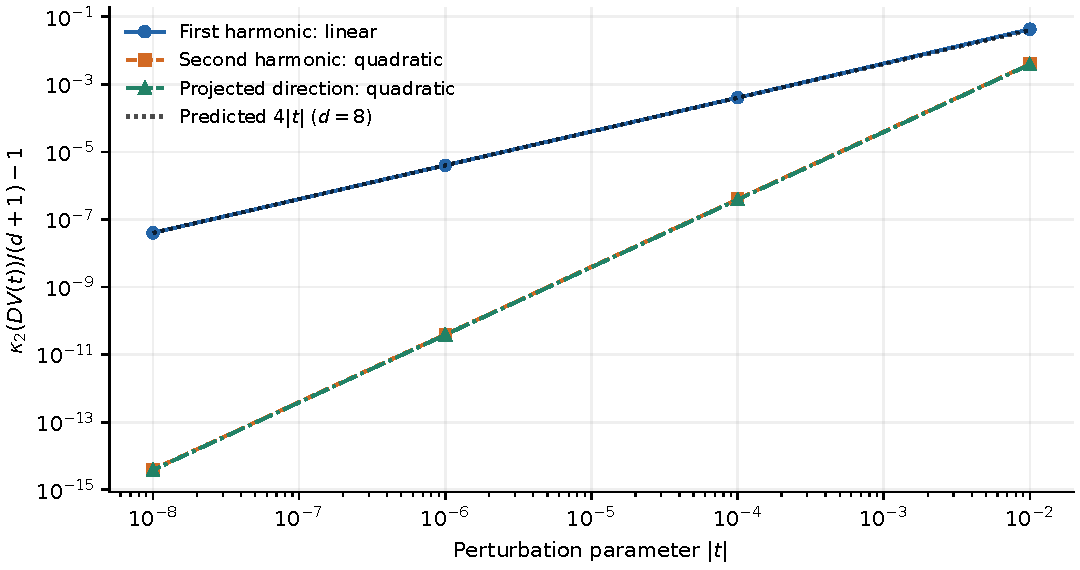
\includegraphics[width=.82\textwidth]{figures/directional_orders.pdf}
\caption{三角权重下的局部条件数增量，$d=8$。第一谐波存在时为一阶；消去第一谐波的非旋转方向为二阶。图中采用80位计算结果。}\label{fig:directions}
\end{figure}

为考察命题\ref{prop:near}上界的松紧，另取 $L=5,9,17$，使用两类正权重：三角权重；以及 $w_{\lfloor L/2\rfloor}=1$、其余 $w_n=2+n/L$ 的内部极小行权重。后一类的最大、最小权重均唯一。为简化记号，将其最小行写为 $j=\lfloor L/2\rfloor$；三角权重取 $j=0$。节点统一为
\[
\beta_k(\varepsilon)=\exp\!\left(\frac{2\pi\mathrm i}{L}(k+\varepsilon q_k)\right),
\qquad q_k=\frac{L(-1)^k-1}{L+1}.
\]
这里 $\sum_kq_k=0$、$\max_k|q_k|=1$，故 $\varepsilon$ 是扰动相对网格间距的最大比例。取
\[
\varepsilon\in\{10^{-12},10^{-10},10^{-8},10^{-6},10^{-4},10^{-3},10^{-2},10^{-1}\},
\]
共48例，并另核验6个 $\varepsilon=0$ 的取等配置。

记式\eqref{eq:moment-bound}的左、右端分别为 $T_j$ 和 $H_{a,b}(\eta)$，对非零扰动报告 $T_j/H_{a,b}(\eta)$。所有算例满足上界。内部极小行权重的比值约为 $0.250$ 至 $0.334$；三角权重中，比值随扰动缩小而明显下降，所测最小值约为 $4.15\times10^{-12}$。两类权重的矩界紧性表现反映了其极值重数的差异。

\begin{figure}[htbp]\centering
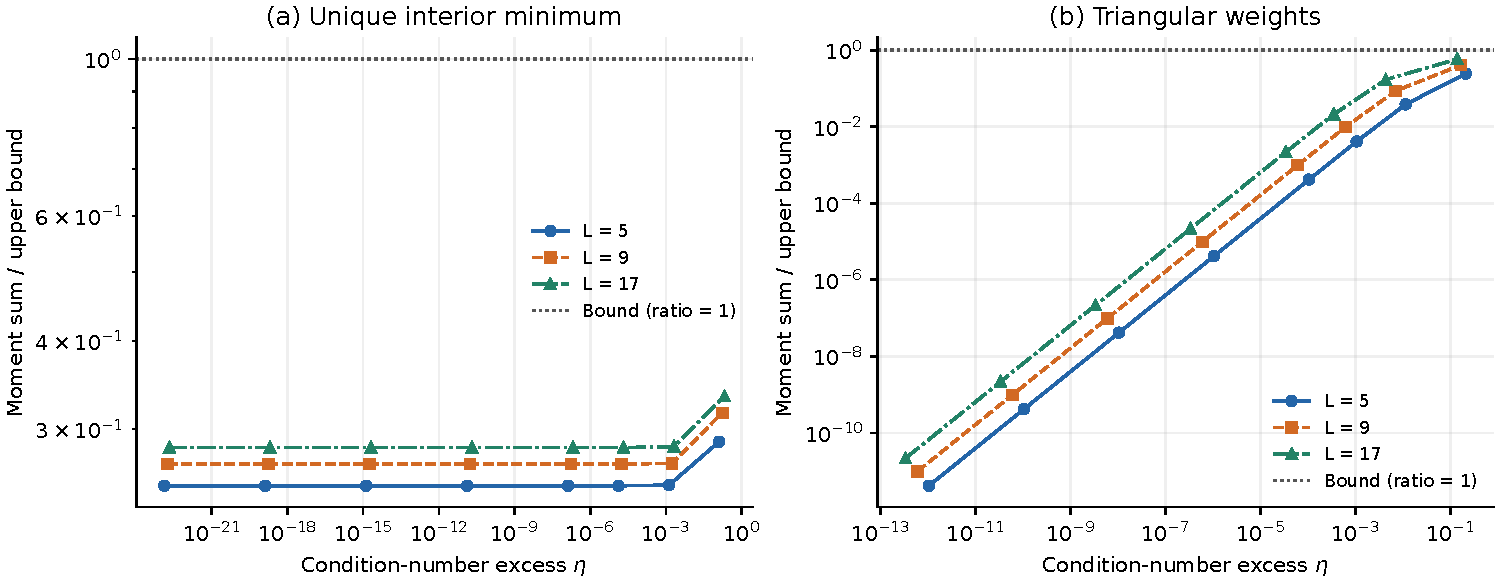
\includegraphics[width=\textwidth]{figures/moment_bound_ratio.pdf}
\caption{近最优矩约束左端与上界之比。每条曲线对应一个固定维数和确定性方向；虚线为比值1。两类权重展示了不同极值重数对应的矩界紧性表现。}\label{fig:moment-ratio}
\end{figure}

这种差别与定理\ref{thm:directional}一致：内部极小行例子的两个极值均唯一，非旋转方向的 $\eta$ 为二阶；三角权重下，该方向的第一谐波非零，$\eta$ 为一阶。两类例子的 $T_j$ 均为二阶，因而前者的比值可以保持非零量级，后者的比值趋于零。

\subsection{计算准确性与批量效率}
定义权重前向误差和系数重构残差
\begin{equation}\label{eq:metrics}
E_\lambda=\frac{\norm{\widehat\lambda-\lambda_{\rm ref}}}{\norm{\lambda_{\rm ref}}},\qquad
R_{\rm dense}=\frac{\norm{\widehat M\widehat\lambda-A}}{\norm A},\qquad
R_{\rm fft}=\frac{\norm{D(L\operatorname{IFFT}(\widehat\lambda))-A}}{\norm A}.
\end{equation}
本文采用 $(\operatorname{IFFT}z)_n=L^{-1}\sum_{k=0}^{L-1}z_k\e^{2\pi\ii nk/L}$ 的归一化约定。

其中 $\lambda_{\rm ref}$ 由80位精度直接 DFT 求和得到，$\widehat M$ 通过浮点节点及逐次幂独立构造。FFT 往返可能共享数值结构，所以不单独以 $R_{\rm fft}$ 证明权重准确性。取 $d=2,8,32,128$，对随机复系数、至多4个非零项的稀疏系数及模长覆盖 $10^{-8}$ 至 $10^8$ 的宽尺度系数各生成3例，共36个算例。

\begin{table}[htbp]\centering\small
\caption{各次数全部9个算例中的最大误差，采用 e 记数法。}\label{tab:accuracy}
\begin{tabular}{rrrrr}\toprule
$d$ & $L$ & $E_\lambda$ & $R_{\rm dense}$ & $R_{\rm fft}$\\\midrule
2 & 5 & 1.40e-16 & 6.31e-16 & 2.93e-16 \\
8 & 17 & 1.74e-16 & 1.53e-14 & 6.43e-16 \\
32 & 65 & 2.47e-16 & 4.85e-14 & 1.07e-15 \\
128 & 257 & 5.17e-16 & 2.61e-13 & 4.96e-15 \\
\\[-.8em]\bottomrule\end{tabular}
\end{table}

理想权重前向误差最大约为 $5.17\times10^{-16}$，独立稠密展开残差最大约为 $2.61\times10^{-13}$。显式节点构造、幂计算和求和增加了舍入误差，三类指标不必相同。另有20个取等输入扰动算例与400个随机算例核验命题\ref{prop:perturb}；取等算例的归一化放大率与1的最大相对差为 $1.52\times10^{-5}$，出现在极小扰动下并包含浮点解相减误差。

批量计时取 $d=8,32,128,512$、$B=1,128$，用相同的 complex128 输入比较 FFT、预计算稠密算子乘法、缓存 LU 求解及每次重新分解后求解。两种 LU 方法使用相同 SciPy 例程和选项。各方法先预热，每组7轮计时中随机排列方法顺序，并设置足够的内部重复以降低计时噪声。图\ref{fig:timing}报告每批在线耗时的中位数，不含输入生成和固定算子准备；重新分解 LU 的在线时间包含分解，缓存 LU 则不包含。准备成本单独列于表\ref{tab:setup}。所有求解结果均与 FFT 权重及稠密重构残差核对。

\begin{table}[htbp]\centering\small
\caption{准备时间中位数，单位为毫秒。各阶段分别计时；缓存 LU 需矩阵构造与分解，稠密变换算子直接构造。}\label{tab:setup}
\begin{tabular}{rrrrr}\toprule
$d$ & 权重 & 矩阵 $M$ & 稠密算子 $R$ & $M$ 的 LU 分解\\\midrule
8 & 0.00396 & 0.0262 & 0.017 & 0.00819 \\
32 & 0.00342 & 0.315 & 0.129 & 0.0507 \\
128 & 0.00492 & 6.91 & 3.58 & 1.75 \\
512 & 0.00632 & 109 & 63.2 & 78.2 \\
\bottomrule\end{tabular}
\end{table}

\begin{figure}[htbp]\centering
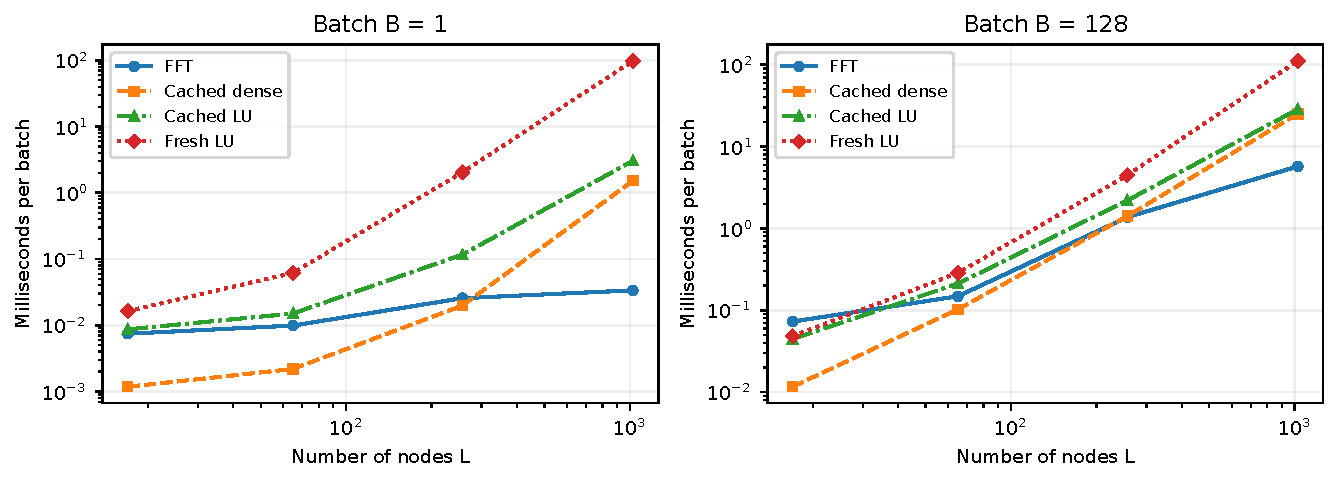
\includegraphics[width=.95\textwidth]{figures/batch_timings.pdf}
\caption{每批在线耗时中位数；左图 $B=1$，右图 $B=128$。两种缓存方法复用准备结果，重新分解 LU 在每次调用中分解矩阵。}\label{fig:timing}
\end{figure}

\FloatBarrier
$d=512$、$B=128$ 时，FFT、缓存稠密变换、缓存 LU 和重新分解 LU 每批分别约为 $5.73$、$25.1$、$28.6$ 和 $111$ ms。小规模时，缓存稠密变换可能比 FFT 更快，排序也随批量大小变化。原始重复计时、准备时间、求解残差与库环境记录见 \texttt{../../code/ela\_revision}；上述结果仅描述所测实现和平台。

\FloatBarrier
\section{讨论与结论}
固定非零单项式行权重时，单位圆上 Vandermonde 矩阵的最优节点恰为旋转后的正多边形。局部 Fourier 判据刻画消除线性增长的方向；当权重模不全相等时，带权矩约束保证每个非旋转平坦方向均有严格二阶增长。式\eqref{eq:general-second}给出每个此类方向的二阶系数，式\eqref{eq:coefficient-lower}给出正下界。三角权重下，一个 Fourier 系数即可决定增长阶数，第二谐波还具有式\eqref{eq:second-harmonic}的显式二阶系数。在注\ref{rem:dimension}的最大角位移归一化下，式\eqref{eq:dimension-coefficient}给出 $C_d\sim2d^2/3$，说明消除线性增长之后仍存在随维数增大的二阶敏感性。

等比平方应用为二元齐次多项式提供固定基底。FFT 公式、Parseval 恒等式与 Kadec 上界使用已有工具；实验核验局部理论，并区分理想权重误差与显式节点重构误差。缓存 LU 与预计算稠密变换为批量计算提供可复用的对照方法，实际耗时优势依赖矩阵规模、批量大小及实现。

待研究的问题包括高阶余项的统一控制、由矩约束推出节点匹配距离，以及实平方因子中的消去误差。

\section*{致谢}
OpenAI ChatGPT（作者提供的模型标签为 ChatGPT 6.1 sol）与 Codex 辅助了中文到英文的翻译、语言润色、文献检索、第3节局部分析的证明推导建议，以及核验、绘图和计时 Python 程序的准备。修订时还参考了 Gemini 和 Grok 生成的初步稿件评议；现有修订材料未记录这两个工具的模型版本。数值记录由随附程序实际计算产生。AI 生成的评议和有限计算不构成独立同行评审或数学证明。人类作者须在投稿前核验论证、文献、代码与计算结果，并对稿件的完整性和原创性负责。

\begingroup\footnotesize\linespread{1.0}\selectfont
\begin{thebibliography}{13}

\bibitem{aubel}
C. Aubel and H. B\"olcskei.
Vandermonde matrices with nodes in the
unit disk and the large sieve.
\emph{Appl. Comput. Harmon. Anal.}, 47:53--86, 2019.

\bibitem{bender}
M. R. Bender, J.-C. Faug\`ere, L. Perret, and E. Tsigaridas.
A nearly optimal algorithm to decompose binary forms.
\emph{J. Symbolic Comput.}, 105:71--96, 2021, \url{https://doi.org/10.1016/j.jsc.2020.06.002}.

\bibitem{berman}
L. Berman and A. Feuer.
On perfect conditioning of Vandermonde
matrices on the unit circle.
\emph{Electron. J. Linear Algebra}, 16:157--161, 2007.

\bibitem{bhatia}
R. Bhatia and C. Davis.
A better bound on the variance.
\emph{Amer. Math. Monthly}, 107:353--357, 2000.

\bibitem{chen}
X. Chen, R. S. Womersley, and J. J. Ye.
Minimizing the condition
number of a Gram matrix.
\emph{SIAM J. Optim.}, 21:127--148, 2011.

\bibitem{summation}
N. J. Higham.
The accuracy of floating point summation.
\emph{SIAM J. Sci. Comput.}, 14:783--799, 1993.

\bibitem{higham}
N. J. Higham.
\emph{Accuracy and Stability of Numerical Algorithms},
2nd ed., SIAM, Philadelphia, 2002.

\bibitem{kuian}
M. Kuian, L. Reichel, and S. V. Shiyanovskii.
Optimally conditioned
Vandermonde-like matrices.
\emph{SIAM J. Matrix Anal. Appl.}, 40:1399--1424, 2019.

\bibitem{pan}
V. Y. Pan.
How bad are Vandermonde matrices?
\emph{SIAM J. Matrix
Anal. Appl.}, 37:676--694, 2016, \url{https://doi.org/10.1137/15M1030170}.

\bibitem{reznick}
B. Reznick.
Some new canonical forms for polynomials.
\emph{Pacific J. Math.}, 266:185--220, 2013.

\bibitem{schatzman}
J. C. Schatzman.
Accuracy of the discrete Fourier transform and the
fast Fourier transform.
\emph{SIAM J. Sci. Comput.}, 17:1150--1166, 1996.

\bibitem{sharma}
R. Sharma and A. Thakur.
More inequalities for positive linear maps.
\emph{J. Math. Inequal.}, 7:1--9, 2013.

\bibitem{yu}
A. Yu and A. Townsend.
On the stability of unevenly spaced samples
for interpolation and quadrature. \emph{BIT Numer. Math.}, 63:Article 23, 2023.

\end{thebibliography}
\endgroup
\end{document}
